\section{Difa Al Fansha}

\subsection{Teori}
	%%Nomor 1
	\subsubsection{Kenapa file suara harus di lakukan MFCC}
	\hfill\\
Machine learning hanya mengerti bilangan vektor saja. MFCC adalah metode untuk memproses sinyal suara. MFCC mengkonversikan data suara menjadi gambar spektrum gelombang, lalu didapatkan lah nilai-nilai dari suara tsb. Nilai-nilai MFCC ini akan dimasukkan langsung kejaringan saraf tiruan, agar dapat diubah menjadi bentuk vektor.
	
	\begin{figure}[H]
		\begin{center}
		 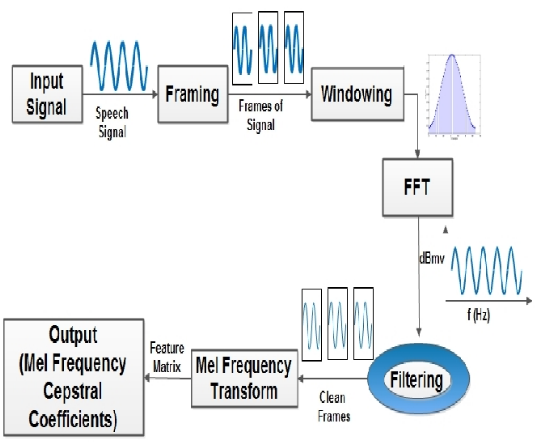
\includegraphics[width=10cm]{figures/1174076/figures6/teori1.png}
		 \caption{Soal 1}	
		\end{center}
	\end{figure}

	%%Nomor 2
	\subsubsection{Konsep dasar neural network}
	\hfill\\
Neural Network ini terinspirasi dari jaringan saraf otak manusia. Dimana setiap neuron terhubung ke setiap neuron di lapisan berikutnya. Lapisan pertama menerima input dan lapisan terakhir memberikan keluaran. Input dari sebuah Neural Network adalah data training(data yang sudah ada). Output adalah data test (data yang dicari).
	
	\begin{figure}[H]
		\begin{center}
		 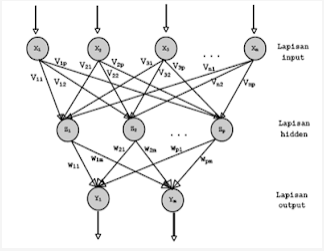
\includegraphics[width=10cm]{figures/1174076/figures6/teori2.png}
		 \caption{Soal 2}	
		\end{center}
	\end{figure}
	 
	%%Nomor 3
	\subsubsection{Konsep pembobotan dalam neural network}
	\hfill\\
Dalam proses neural network mulai dari input yang diterima oleh neuron bersama dengan nilai bobot masing-masing input. Setelah memasuki neuron, nilai input akan ditambahkan oleh fungsi penerima. Hasil penambahan ini akan diproses oleh masing-masing fungsi neuron, hasil penambahan ini akan dibandingkan dengan nilai ambang tertentu. Semakin besar bobot sebuah input, maka sinyal yang berasal dari input tertentu memiliki prioritas yang semakin besar untuk bisa berkontribusi kepada neuron di depannya. Selain itu, bobot juga menentukan apakah sinyal dari input tertentu bisa melewati neuron di depannya atau tidak.

	\begin{figure}[H]
		\begin{center}
		 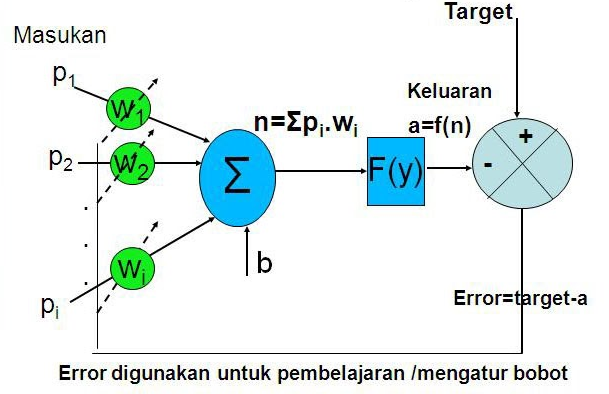
\includegraphics[width=10cm]{figures/1174076/figures6/teori3.png}
		 \caption{Soal 3}	
		\end{center}
	\end{figure}
	 
	%%Nomor 4
	\subsubsection{Konsep fungsi aktifasi dalam neural network}
	\hfill\\
	Fungsi aktivasi merupakan operasi matematik yang digunakan untuk mendapatkan output neuron dari nilai inputnya. Terdapat beberapa fungsi aktivasi, lihat pada gambar berikut :

	\begin{figure}[H]
		\begin{center}
		 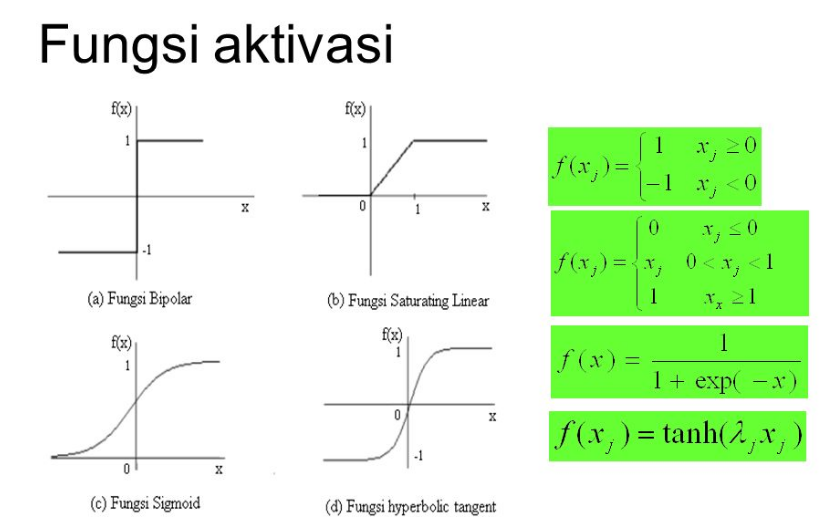
\includegraphics[width=10cm]{figures/1174076/figures6/teori4.png}
		 \caption{Soal 4}	
		\end{center}
	\end{figure}	
	
	%%Nomor 5
	\subsubsection{Cara membaca hasil plot dari MFCC} 
	\hfill\\
	\begin{figure}[H]
		\begin{center}
		 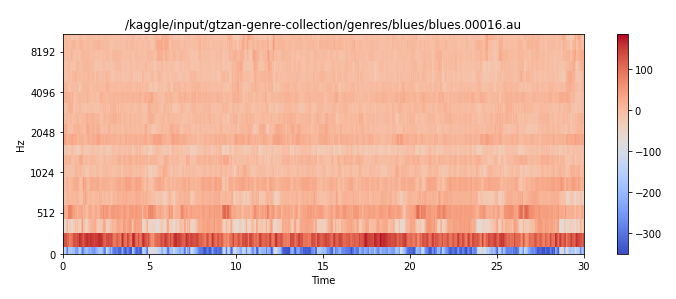
\includegraphics[width=10cm]{figures/1174076/figures6/teori5.png}
		 \caption{Soal 5}	
		\end{center}
	\end{figure}	
	
	\hfill\\
	Dari gambar soal 5 dapat diketahui :
	\begin{itemize}
		\item Terdapat 2 dimensi yaitu x sebagai waktu, dan y sebagai power atau desibel.
		\item Dapat dilihat bahwa jika berwarna biru maka power dari suara tersebut rendah, dan jika merah power dari suara tersebut tinggi
		\item Dibagian atas terdapat warna merah pudar yang menandakan bahwa tidak ada suara sama sekali dalam jangkauan tersebut.
	\end{itemize}
	 
	%%Nomor 6
	\subsubsection{one-hot encoding}
	\hfill\\
Proses memetakan kata-kata ke dalam angka biner.

	\begin{figure}[H]
		\begin{center}
		 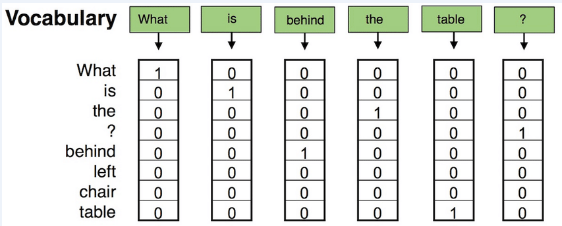
\includegraphics[width=10cm]{figures/1174076/figures6/teori6.png}
		 \caption{Soal 6}	
		\end{center}
	\end{figure}
	 
	%%Nomor 7
	\subsubsection{Apa fungsi dari np.unique dan to categorical dalam kode program}
	\hfill\\
Mengembalikkan array yang unik(data yang berbeda), function ini akan mengambil isi array yang berbeda.

	\begin{figure}[H]
		\begin{center}
		 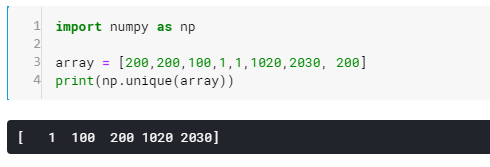
\includegraphics[width=10cm]{figures/1174076/figures6/teori7.png}
		 \caption{Soal 7}	
		\end{center}
	\end{figure}
	
	\begin{figure}[H]
		\begin{center}
		 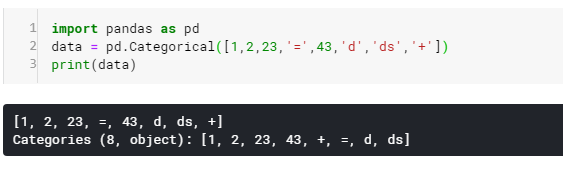
\includegraphics[width=10cm]{figures/1174076/figures6/teori7_2.png}
		 \caption{Soal 7}	
		\end{center}
	\end{figure}
	 
	%%Nomor 8
	\subsubsection{Apa fungsi dari Sequential dalam kode program}
	\hfill\\
	Fungsi dari Sequential sebagai salah satu jenis model yang digunakan dalam perhitungan. Sequential ini membangun tumpukan linear yang berurutan.
	\begin{figure}[H]
		\begin{center}
		 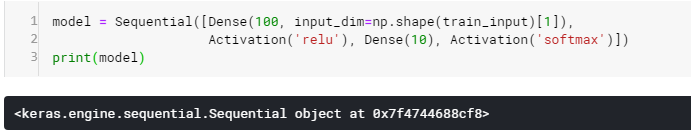
\includegraphics[width=10cm]{figures/1174076/figures6/teori8.png}
		 \caption{Soal 7}	
		\end{center}
	\end{figure}
	
\subsection{Praktek}
 
	%%Nomor 1
	\subsubsection{Jelaskan isi dari data GTZAN Genre Collection dan data dari freesound. Buat kode program untuk meload data tersebut untuk digunakan pada MFCC. Jelaskan arti dari setiap baris kode yang dibuat(harus beda dengan teman sekelas)}
\hfill\\
Data GTZAN Genre Collection berisikan 1000 lagu dari 10 genre berbeda. Ditiap genrenya masing-masing terdapat 100 lagu yang kurang lebih durasinya 30 detik.

	\lstinputlisting[firstline=7, lastline=28]{src/1174076/src6/1174076.py}
	
	\begin{figure}[H]
		\begin{center}
		 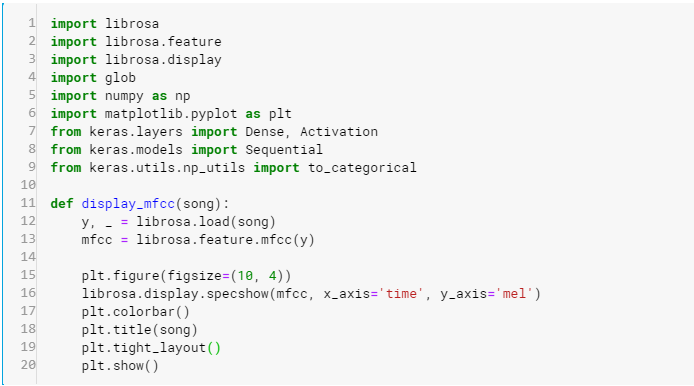
\includegraphics[width=10cm]{figures/1174076/figures6/praktek1.png}
		 \caption{Praktek 1}	
		\end{center}
	\end{figure}
 
	%%Nomor 2
	\subsubsection{Jelaskan perbaris kode program dengan kata-kata dan dilengkapi ilustrasi gambar fungsi dari display\_mfcc()}
\hfill\\

	\lstinputlisting[firstline=29, lastline=52]{src/1174076/src6/1174076.py}
	
	\begin{figure}[H]
		\begin{center}
		 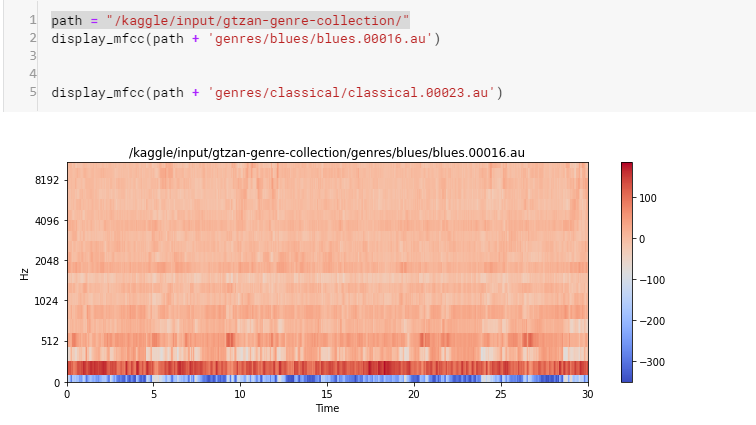
\includegraphics[width=10cm]{figures/1174076/figures6/praktek2.png}
		 \caption{Praktek 2}	
		\end{center}
	\end{figure}
 
 
	%%Nomor 3
\subsubsection{Jelaskan perbaris kode program dengan kata-kata dan dilengkapi ilustrasi gambar fungsi dari extract\_features\_song(). Jelaskan juga mengapa yang diambil 25.000 baris pertama?}
\hfill\\
Alasan diambil 25000 baris pertama, karena setiap lagu memiliki panjang nilai MFCC yang berbeda-beda dan yang dimasukkan ke dalam neuron harus memiliki ukuran yang sama.

	\lstinputlisting[firstline=54, lastline=63]{src/1174076/src6/1174076.py}
	
	\begin{figure}[H]
		\begin{center}
		 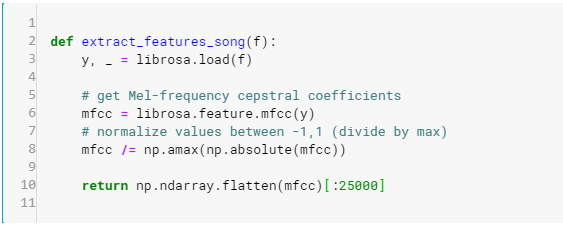
\includegraphics[width=10cm]{figures/1174076/figures6/praktek3.png}
		 \caption{Praktek 3}	
		\end{center}
	\end{figure}
 
	%%Nomor 4
\subsubsection{Jelaskan perbaris kode program dengan kata-kata dan dilengkapi ilustrasi gambar fungsi dari generate\_features\_and\_labels()}
\hfill\\

	\lstinputlisting[firstline=65, lastline=83]{src/1174076/src6/1174076.py}
	
	\begin{figure}[H]
		\begin{center}
		 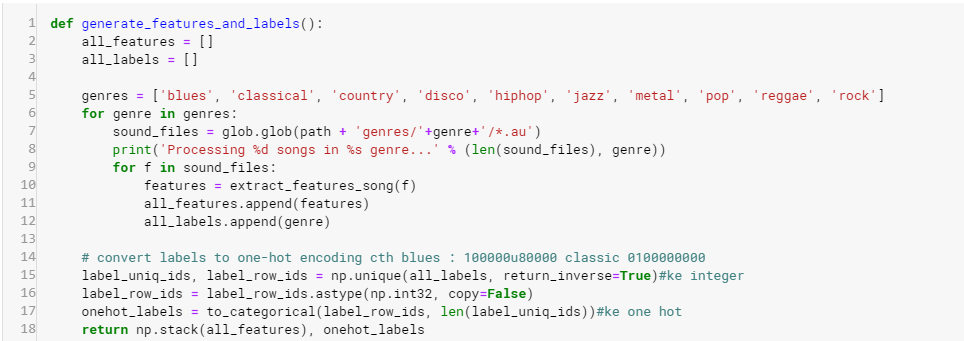
\includegraphics[width=10cm]{figures/1174076/figures6/praktek4.png}
		 \caption{Praktek 4}	
		\end{center}
	\end{figure}
 
 
	%%Nomor 5
\subsubsection{Jelaskan dengan kata dan praktek kenapa penggunaan fungsi generate\_features\_and\_labels() sangat lama ketika meload dataset genre. Tunjukkan keluarannya dari komputer sendiri dan artikan maksud setiap luaran yang didapatkan}
\hfill\\

	\lstinputlisting[firstline=85, lastline=89]{src/1174076/src6/1174076.py}

	\begin{figure}[H]
		\begin{center}
		 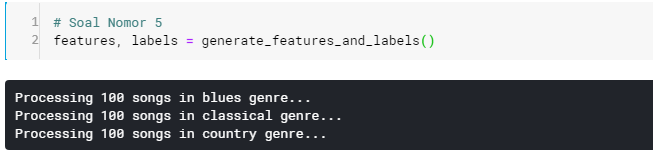
\includegraphics[width=10cm]{figures/1174076/figures6/praktek5.png}
		 \caption{Praktek 5}	
		\end{center}
	\end{figure}
	
	\begin{figure}[H]
		\begin{center}
		 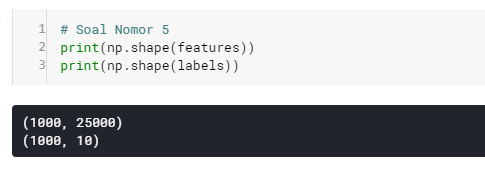
\includegraphics[width=10cm]{figures/1174076/figures6/praktek5_2.png}
		 \caption{Praktek 5.2}	
		\end{center}
	\end{figure}
 
 	 
	%%Nomor 6
\subsubsection{Jelaskan kenapa harus dilakukan pemisahan data training dan data set sebesar 80\%? Praktekkan dengan kode dan Tunjukkan keluarannya dari komputer sendiri dan artikan maksud setiap luaran yang didapatkan}
\hfill\\
Dilakukannya pemisahan data training dan data set sebesar 80\% agar model yang dihasilkan lebih akurat dan meminimalisir kesalahan dalam pembelajaran mesin.

	\lstinputlisting[firstline=91, lastline=110]{src/1174076/src6/1174076.py}
	
	\begin{figure}[H]
		\begin{center}
		 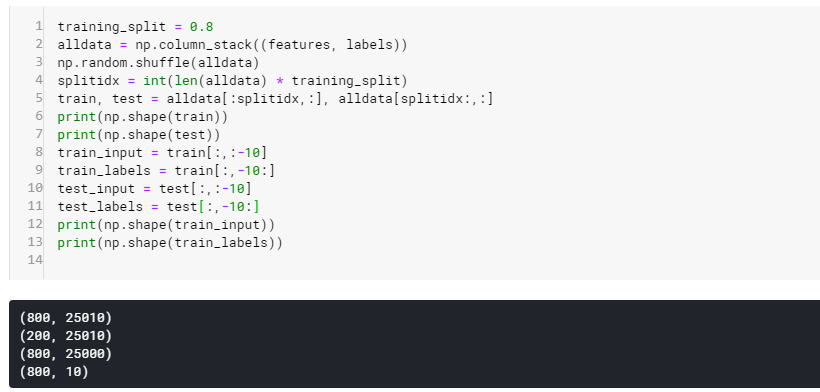
\includegraphics[width=10cm]{figures/1174076/figures6/praktek6.png}
		 \caption{Praktek 6}	
		\end{center}
	\end{figure}
 
	%%Nomor 7
\subsubsection{Praktekkan dan jelaskan masing-masing parameter dari fungsi Sequential(). Tunjukkan keluaranya dari komputer sendiri dan artikan maksud setiap luaran yang didapatkan}
\hfill\\

\lstinputlisting[firstline=112, lastline=118]{src/1174076/src6/1174076.py}
	 
	\begin{figure}[H]
		\begin{center}
		 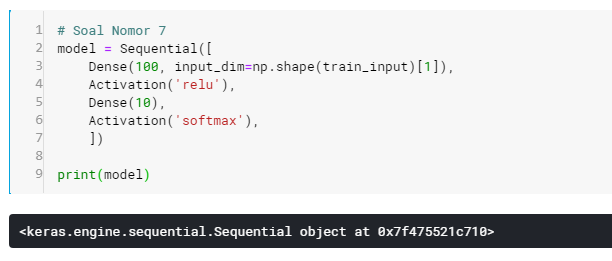
\includegraphics[width=10cm]{figures/1174076/figures6/praktek7.png}
		 \caption{Praktek 7}	
		\end{center}
	\end{figure}
 
	%%Nomor 8
\subsubsection{Praktekkan dan jelaskan masing-masing parameter dari fungsi Sequential(). Tunjukkan keluaranya dari komputer sendiri dan artikan maksud setiap luaran yang didapatkan}
\hfill\\

\lstinputlisting[firstline=120, lastline=124]{src/1174076/src6/1174076.py}
	 
	\begin{figure}[H]
		\begin{center}
		 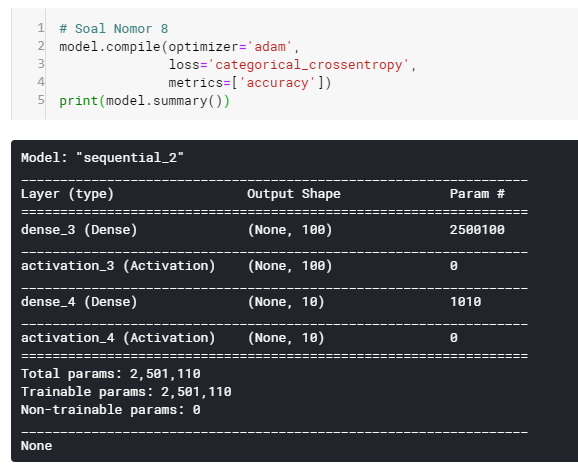
\includegraphics[width=10cm]{figures/1174076/figures6/praktek8.png}
		 \caption{Praktek 8}	
		\end{center}
	\end{figure}
 
	%%Nomor 9
\subsubsection{Praktekkan dan jelaskan masing-masing parameter dari fungsi compile(). Tunjukkan keluaranya dengan fungsi summary dari komputer sendiri dan artikan maksud setiap luaran yang didapatkan}
\hfill\\

\lstinputlisting[firstline=126, lastline=128]{src/1174076/src6/1174076.py}
	 
	\begin{figure}[H]
		\begin{center}
		 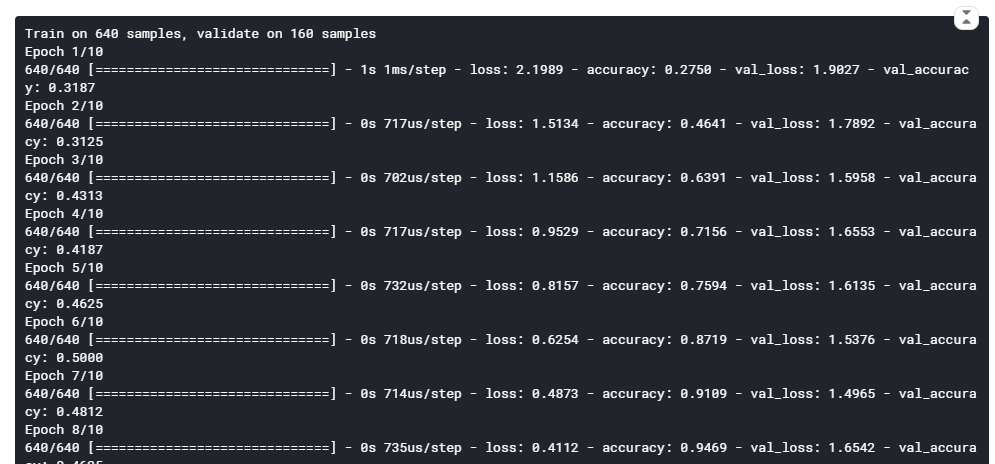
\includegraphics[width=10cm]{figures/1174076/figures6/praktek9.png}
		 \caption{Praktek 9}	
		\end{center}
	\end{figure}
 
	%%Nomor 10
\subsubsection{Praktekkan dan jelaskan masing-masing parameter dari fungsi fit(). dan tunjukkan maksud setiap luaran yang didapatkan}
\hfill\\

\lstinputlisting[firstline=130, lastline=134]{src/1174076/src6/1174076.py}
	
	\begin{figure}[H]
		\begin{center}
		 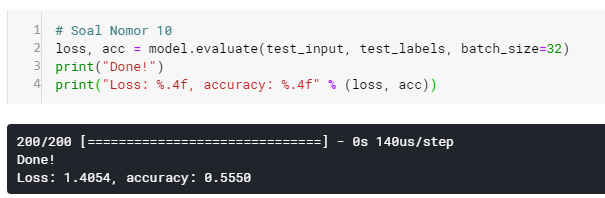
\includegraphics[width=10cm]{figures/1174076/figures6/praktek10.png}
		 \caption{Praktek 10}	
		\end{center}
	\end{figure}
 
	%%Nomor 11
\subsubsection{Praktekkan dan jelaskan masing-masing parameter dari fungsi evaluate(). Tunjukkan keluaranya dari komputer sendiri dan artikan maksud setiap luaran yang didapatkan}
\hfill\\

\lstinputlisting[firstline=136, lastline=137]{src/1174076/src6/1174076.py}

	\begin{figure}[H]
		\begin{center}
		 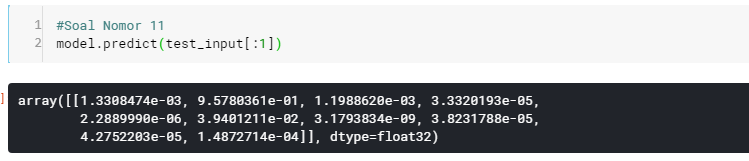
\includegraphics[width=10cm]{figures/1174076/figures6/praktek11.png}
		 \caption{Praktek 11}	
		\end{center}
	\end{figure}
 
\subsection{Penangan Error}
	
	\subsubsection{Screenshoots Error}\hfill\\
	
	\begin{figure}[H]
		\begin{center}
		 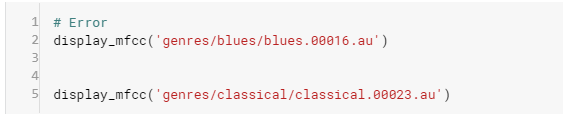
\includegraphics[width=10cm]{figures/1174076/figures6/error1.png}
		 \caption{Error}	
		\end{center}
	\end{figure}
	
	\begin{figure}[H]
		\begin{center}
		 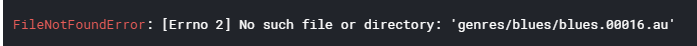
\includegraphics[width=10cm]{figures/1174076/figures6/error2.png}
		 \caption{Kode Error}	
		\end{center}
	\end{figure}
	
	
	\subsubsection{Tuliskan kode eror dan jenis errornya}\hfill\\
		\begin{itemize}
		\item Kode Error : Errno 2
		
		\item Jenis Error : No such file or directory
		
		\end{itemize}
	 
	\subsubsection{Solusi pemecahan masalah error tersebut}\hfill\\
	
	\begin{figure}[H]
		\begin{center}
		 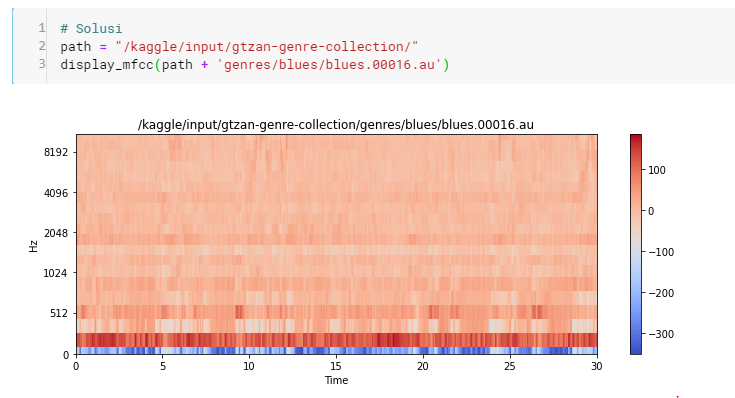
\includegraphics[width=10cm]{figures/1174076/figures6/solusi.png}
		 \caption{Solusi}	
		\end{center}
	\end{figure}
	
	
\subsection{Link Youtube}
	
	\subsubsection{}\hfill\\
	